\chapter{Background and Related Work}\label{sec:literature-review}

\paragraph{Scope relative to the canonical model.}
Unless stated otherwise, the relay-processing methods reviewed in this chapter
are discussed in the context of the canonical matched, memoryless, uncoded
two-hop SISO model used in Chapter~\ref{sec:experiments}: complex-baseband
Gray-coded QPSK over i.i.d.\ Rayleigh fast fading, with coherent receiver-side
processing. BPSK/AWGN formulas are retained only as analytical calibration or
companion special cases. Channel memory, sequence detection, and uncertainty
in the channel description are background for the deliberately non-canonical
experiments of Chapter~\ref{sec:unknown-channels}. The coded material in
Section~\ref{sec:channel-coding-background} supports the supplementary
coded/resource study and is separate from the four-layer information ladder.

\section{Classical Relay Strategies}\label{sec:classical-relay-strategies}

The question motivating this thesis is not whether a learned relay universally
supersedes classical processing, but under which conditions it can complement
it. Classical rules are preferred when their model is identifiable and their
exact processing is affordable; learned relaying is of interest when per-block
identification is unreliable or unavailable, or when exact model-based
processing exceeds the arithmetic or resource budget.

\subsection{Amplify-and-Forward (AF)}
\label{sec:classical-relay-strategies-af}

The AF relay amplifies the received signal by a gain factor \(G\) that
normalizes the output power:
\begin{equation}\protect\phantomsection\label{eq:af-gain}
G =
\sqrt{\frac{P_{\mathrm{target}}}
{\mathbb{E}\!\left[\lVert y_R\rVert^2\right]}} .
\end{equation}
\addcontentsline{equ}{listequations}
{\protect\numberline{\theequation}\quad af-gain}

The standard end-to-end SNR expression for CSI-assisted variable-gain AF is
\cite{Laneman2004CooperativeDiversity,TseViswanath2005Fundamentals}
\begin{equation}\protect\phantomsection\label{eq:af-snr}
\mathrm{SNR}_{\mathrm{eff}}^{\mathrm{AF}}
=
\frac{\mathrm{SNR}_1\mathrm{SNR}_2}
{\mathrm{SNR}_1+\mathrm{SNR}_2+1}.
\end{equation}
\addcontentsline{equ}{listequations}
{\protect\numberline{\theequation}\quad af-snr}

This form assumes that the relay updates its gain from instantaneous first-hop
CSI. It is not the closed form of the power-normalized fixed-gain
implementation used in the simulations, whose gain is a block-level scalar
based on empirical received power. Equation~\ref{eq:af-snr} is therefore
retained as standard background illustrating the familiar bottleneck and
noise-amplification effects, not as an analytic curve for the simulated AF
relay.

\subsection{Decode-and-Forward (DF)}
\label{sec:classical-relay-strategies-df}

The symbol-wise DF relay demodulates the received sample and re-modulates the
resulting bits:
\begin{equation}\protect\phantomsection\label{eq:df-demod-remod}
\hat b_R=\mathrm{demod}(y_R),
\qquad
x_R=\mathrm{mod}(\hat b_R).
\end{equation}
\addcontentsline{equ}{listequations}
{\protect\numberline{\theequation}\quad df-demod-remod}

If the two hop errors are independent and a pair of bit flips cancels, the
end-to-end BER is
\begin{equation}\protect\phantomsection\label{eq:df-ber-hops}
P_e^{\mathrm{DF}}
=
P_{e,1}(1-P_{e,2})+(1-P_{e,1})P_{e,2}.
\end{equation}
\addcontentsline{equ}{listequations}
{\protect\numberline{\theequation}\quad df-ber-hops}

Thus
\(P_e^{\mathrm{DF}}=P_{e,1}+P_{e,2}-2P_{e,1}P_{e,2}\).
For the BPSK/AWGN companion convention of
Section~\ref{sec:awgn-channel-theoretical-analysis},
\(P_e=Q(\sqrt{\mathrm{SNR}})\) per hop. The canonical benchmark is instead
Gray-coded QPSK over Rayleigh fading, for which coherent componentwise slicing
is applied after equalization and the QPSK \(E_s/N_0\)-to-\(E_b/N_0\)
conversion must be made.

The term DF also denotes an information-theoretic coded block strategy: the
relay decodes a message block protected by a channel code, then re-encodes and
forwards it. That strategy is distinct from the uncoded symbol-wise baseline
above. In the matched memoryless per-symbol setting, coherent nearest-neighbor
QPSK slicing is the MAP hard decision for each symbol; this does not make
symbol-wise DF globally optimal over coded, block, soft, sequence, or
end-to-end relay mappings.

\subsection{Other Classical Relay Techniques}

AF and DF are canonical reference protocols, while compress-and-forward,
estimate-and-forward, and compute-and-forward occupy other points in the relay
design space. They are background only here. AF and symbol-wise DF are
representative baselines for the specified two-hop benchmark, not universal
lower and upper bounds, and memoryless AF/DF failure under ISI must not be
generalized to correctly informed sequence detection.

\section{Machine Learning in Wireless Communication}
\label{sec:machine-learning-in-wireless-communication}

Deep learning has been applied to channel estimation
\cite{YeLiJuang2018OFDMDL}, signal detection
\cite{SamuelDiskinWunder2019MIMODetect}, end-to-end communication
\cite{Dorner2018OverTheAirDL}, and resource allocation
\cite{Sun2018LearnToOptimize}. These studies motivate learned physical-layer
mappings when an analytical model is unavailable, mismatched, or expensive to
use; they do not imply that a learned receiver dominates a correctly matched
and affordable one.

\subsection{Theoretical Basis: Universal Approximation and Denoising}
\label{sec:theoretical-basis-universal-approximation-and-denoising}

The universal approximation theorem
\cite{GoodfellowBengioCourville2016DeepLearning} states that a sufficiently
wide feedforward network with a non-linear activation can approximate
continuous functions on compact domains. For a real decision component, a
denoising target may be written
\begin{equation}\protect\phantomsection\label{eq:optimal-denoiser}
f^*:\mathbb{R}^{2w+1}\rightarrow[-1,1],
\qquad
f^*(y_{i-w:i+w})
=
\mathbb{E}[x_i\mid y_{i-w:i+w}].
\end{equation}
\addcontentsline{equ}{listequations}
{\protect\numberline{\theequation}\quad optimal-denoiser}

This conditional expectation is the Bayes-optimal MSE estimator under the
stated distribution. For equiprobable BPSK in the real-AWGN companion model,
\begin{equation}\protect\phantomsection\label{eq:optimal-denoiser-awgn}
f^*(y)=\tanh\!\left(\frac{y}{\sigma^2}\right).
\end{equation}
\addcontentsline{equ}{listequations}
{\protect\numberline{\theequation}\quad optimal-denoiser-awgn}

The same binary posterior-mean form applies per independent axis of coherently
processed QPSK only after the appropriate conditional noise scaling is
specified. A single tanh unit represents the fixed-variance BPSK/AWGN
expression exactly, but a relay trained over several SNRs and fading
realizations approximates a family of conditional maps rather than one fixed
posterior.

The bias--variance decomposition provides general background for model sizing:
\begin{equation}\protect\phantomsection\label{eq:bias-variance-decomp}
\mathbb{E}[(\hat x-x)^2]
=
\mathrm{Bias}^2(\hat x)+\mathrm{Var}(\hat x)
+\sigma^2_{\mathrm{irreducible}}.
\end{equation}
\addcontentsline{equ}{listequations}
{\protect\numberline{\theequation}\quad bias-variance-decomp}

It motivates asking whether extra capacity reduces approximation bias,
increases estimator variance, or simply remains unused. It does not establish
excess-capacity overfitting in this thesis. The final evidence supports
saturation or idle capacity over the swept range and shows that required
context, rather than parameter count alone, is binding on channels with memory.

\subsection{Prior Work in Deep Learning for Physical-Layer Processing}
\label{sec:prior-work-in-deep-learning-for-physical-layer-processing}

Ye et al.~\cite{YeLiJuang2018OFDMDL} use deep networks for joint channel
estimation and detection in OFDM. Samuel et
al.~\cite{SamuelDiskinWunder2019MIMODetect} propose DetNet, which unfolds an
iterative MIMO detector. Dorner et al.~\cite{Dorner2018OverTheAirDL} formulate
the transmitter, channel, and receiver as an end-to-end autoencoder, while Sun
et al.~\cite{Sun2018LearnToOptimize} apply learning to resource allocation.

In relay-assisted systems, many learning studies address relay selection or
resource allocation while retaining conventional forwarding
\cite{Akdemir2024DLRelaySelection}. Related work also treats relay networks as
trainable nonlinear processing graphs or optimizes analog relay gains
\cite{Gunduz2019MLAir,Bergel2023RelaysAsNeurons,BergelICASSP2024}.
These problems differ from learning the symbol-level relay input--output map.
Classical AF/DF frameworks remain the reference background
\cite{Nosratinia2004CooperativeCommunication}; the relevant comparison depends
on whether the classical model and the information needed to run it are
available.

\subsection{Neural Network Relay Processing}
\label{sec:neural-network-relay-processing}

A supervised relay can be trained by empirical MSE:
\begin{equation}\protect\phantomsection\label{eq:mse-loss}
\mathcal{L}(\theta)
=
\frac{1}{N}\sum_{i=1}^{N}(\hat x_i-x_i)^2,
\qquad
\hat x_i=f_\theta(y_{i-w:i+w}).
\end{equation}
\addcontentsline{equ}{listequations}
{\protect\numberline{\theequation}\quad mse-loss}

A two-layer MLP instance is
\begin{equation}\protect\phantomsection\label{eq:mlp-relay}
\mathbf h
=
\mathrm{ReLU}(\mathbf W_1\mathbf w+\mathbf b_1),
\qquad
\hat x
=
\tanh(\mathbf W_2\mathbf h+\mathbf b_2).
\end{equation}
\addcontentsline{equ}{listequations}
{\protect\numberline{\theequation}\quad mlp-relay}

Under the canonical i.i.d.\ fast-fading, white-noise model, neighboring samples
contain no additional sufficient information about \(x_i\) after coherent
compensation; \(w=0\) is sufficient. A finite window is an architectural
convention there, not a source of extra information. On a channel with memory,
by contrast, the useful context must span the interference. A symmetric window
also reads \(w\) future samples in streaming operation. Whole-block buffering
in the studied half-duplex protocol can absorb that look-ahead, but it remains
structural latency for a streaming relay.

Multi-SNR training fits one fixed estimator over the sampled SNR distribution.
It is amortized within-family inference, not online adaptation, minimax
protection, or evidence of generalization to structurally unseen channel
families. Learned inference cost is fixed only after the architecture, window,
input/output dimensions, and modulation interface are fixed; widening context
or outputs can increase cost.

\section{Generative Models for Signal Processing}
\label{sec:generative-models-for-signal-processing}

Generative models represent distributions rather than only point mappings.
Formally,
\begin{equation}\protect\phantomsection\label{eq:bayes-rule}
p(\mathbf x\mid\mathbf y)
\propto
p(\mathbf y\mid\mathbf x)p(\mathbf x).
\end{equation}
This factorization can separate a signal prior from an observation model, but
by itself does not guarantee robustness to noise processes or channel families
absent from training.

\subsection{Variational Autoencoders}\label{sec:variational-autoencoders}

A variational autoencoder (VAE) \cite{KingmaWelling2014VAE} introduces a latent
variable \(\mathbf z\sim\mathcal N(\mathbf 0,\mathbf I)\), a decoder
\(p_\theta(\mathbf x\mid\mathbf z)\), and an approximate posterior
\(q_\phi(\mathbf z\mid\mathbf x)\). The log evidence decomposes as
\begin{equation}\protect\phantomsection\label{eq:vae-elbo}
\log p_\theta(\mathbf x)
=
\underbrace{
\mathbb E_{q_\phi}\!\left[
\log\frac{p_\theta(\mathbf x,\mathbf z)}
{q_\phi(\mathbf z\mid\mathbf x)}
\right]}_{\mathrm{ELBO}(\theta,\phi;\mathbf x)}
+
\underbrace{
D_{\mathrm{KL}}\!\left(
q_\phi(\mathbf z\mid\mathbf x)
\Vert
p_\theta(\mathbf z\mid\mathbf x)
\right)}_{\ge 0}.
\end{equation}
\addcontentsline{equ}{listequations}
{\protect\numberline{\theequation}\quad vae-elbo}

A common \(\beta\)-VAE objective is
\begin{equation}\protect\phantomsection\label{eq:vae-loss}
\mathcal L_{\mathrm{VAE}}
=
\mathbb E_{q_\phi(\mathbf z\mid\mathbf x)}
[\log p_\theta(\mathbf x\mid\mathbf z)]
-
\beta D_{\mathrm{KL}}\!\left(
q_\phi(\mathbf z\mid\mathbf x)\Vert p(\mathbf z)
\right),
\end{equation}
where \(\beta\) trades reconstruction against latent regularity
\cite{Higgins2017betaVAE}. The reparameterization trick writes
\begin{equation}\protect\phantomsection\label{eq:repremtrized-trick}
\mathbf z
\sim
\mathcal N(\boldsymbol\mu,\mathrm{diag}(\boldsymbol\sigma^2)),
\end{equation}
\begin{equation}\protect\phantomsection
\label{eq:repremtrized-trick-resample}
\mathbf z
=
\boldsymbol\mu+\boldsymbol\sigma\odot\boldsymbol\epsilon,
\qquad
\boldsymbol\epsilon\sim\mathcal N(\mathbf 0,\mathbf I).
\end{equation}
Sampling at inference adds variance to a point estimate; substituting the
latent mean is a different read-out. The literature background alone does not
determine which is preferable for relay denoising.

\subsection{Conditional Generative Adversarial Networks}
\label{sec:conditional-generative-adversarial-networks}

Conditional GANs \cite{MirzaOsindero2014cGAN} train a generator conditioned on
the noisy observation against a discriminator or critic that distinguishes
generated from clean samples. WGAN-GP \cite{Gulrajani2017WGANgp} replaces the
saturating adversarial objective with a Wasserstein critic and a gradient
penalty enforcing an approximate Lipschitz constraint. In the implemented
relay, an additional reconstruction term makes the system primarily a
conditioned denoiser with adversarial regularization. This architecture is
background here; no universal robustness or efficiency claim follows from the
generative formulation.

\subsection{Generative vs.\ Discriminative Paradigms for Relay Processing}
\label{sec:generative-vs.-discriminative-paradigms-for-relay-processing}

Generative and discriminative relays impose different inductive biases. For
QPSK processed per axis, each clean component has a binary support; the
analogous BPSK support is likewise simple. This makes the added generative
machinery a question for controlled evaluation rather than a presumed
advantage or disadvantage. Detailed thesis-specific BER comparisons remain in
the experimental chapters.

\section{Sequence Models: Transformers, State Space Models}
\label{sec:sequence-models-transformers-and-state-space-models}

Transformers and structured state-space models provide different mechanisms
for using context. Their algorithmic properties motivate comparison on signals
with memory, but neither architecture is expected to gain information from
redundant neighboring samples on the canonical memoryless channel.

\subsection{Transformers and the Attention Mechanism}
\label{sec:transformers-and-the-attention-mechanism}

Transformers \cite{Vaswani2017Attention} use self-attention
\begin{equation}\protect\phantomsection\label{eq:attention}
\mathrm{Attention}(\mathbf Q,\mathbf K,\mathbf V)
=
\mathrm{softmax}\!\left(
\frac{\mathbf Q\mathbf K^T}{\sqrt{d_k}}
\right)\mathbf V.
\end{equation}

Multi-head attention applies independent projections and concatenates their
outputs:
\begin{equation}\protect\phantomsection\label{eq:multihead-attention}
\begin{aligned}
\mathrm{MultiHead}(\mathbf X)
&=
\mathrm{Concat}(\mathrm{head}_1,\ldots,\mathrm{head}_h)\mathbf W^O,\\
\mathrm{head}_i
&=
\mathrm{Attention}(
\mathbf X\mathbf W_i^Q,
\mathbf X\mathbf W_i^K,
\mathbf X\mathbf W_i^V).
\end{aligned}
\end{equation}

The four dense projection matrices contribute
\begin{equation}\protect\phantomsection
\label{eq:multihead-attention-parameters-count}
3d_{\mathrm{model}}^2+d_{\mathrm{model}}^2
=
4d_{\mathrm{model}}^2
\end{equation}
parameters in the square-projection case, and the \(n\times n\) attention matrix
\begin{equation}\protect\phantomsection
\label{eq:multihead-attention-matrix}
\mathbf A
=
\mathrm{softmax}\!\left(
\frac{\mathbf Q\mathbf K^T}{\sqrt{d_k}}
\right)
\end{equation}
has quadratic time and memory scaling in sequence length for standard dense
attention. At the short windows studied here, this asymptotic distinction is
not by itself a latency result. Sinusoidal positional encoding is
\begin{equation}\protect\phantomsection\label{eq:positional-encoding}
PE_{(pos,2k)}
=
\sin\!\left(\frac{pos}{10000^{2k/d}}\right),
\qquad
PE_{(pos,2k+1)}
=
\cos\!\left(\frac{pos}{10000^{2k/d}}\right).
\end{equation}

\subsection{Structured State Space Models}
\label{sec:structured-state-space-models}

Structured state-space models (SSMs) \cite{GuGoelRe2022SSM} discretize a
linear dynamical system. With zero-order hold,
\begin{equation}\protect\phantomsection\label{eq:ssm-discrete}
\mathbf x_k
=
\bar{\mathbf A}\mathbf x_{k-1}+\bar{\mathbf B}u_k,
\qquad
y_k=\mathbf C\mathbf x_k+Du_k,
\qquad
\bar{\mathbf A}=e^{\Delta\mathbf A}.
\end{equation}
HiPPO-based initialization and structured or diagonal-plus-low-rank state
matrices make long recurrences tractable, and S4 uses this structure to obtain
linear scaling in sequence length \cite{GuGoelRe2022SSM}. These are algorithmic
properties; they do not establish end-to-end relay latency or superiority over
attention at the short contexts evaluated in this thesis.

\subsection{Mamba and Mamba-2}\label{sec:mamba-selective-state-spaces}

Mamba \cite{gu2023mamba} makes selected SSM parameters input-dependent:
\begin{equation}\protect\phantomsection\label{eq:mamba-selective}
\Delta_k
=
\mathrm{softplus}(W_\Delta u_k+b_\Delta),
\qquad
\mathbf B_k=W_Bu_k,
\qquad
\mathbf C_k=W_Cu_k.
\end{equation}
With a stable diagonal \(\mathbf A\), changing \(\Delta_k\) controls how
strongly the state is retained or refreshed. This selectivity can be
interpreted as adaptive filtering, but only as an architectural capability: on
the canonical memoryless channel there is no temporal state needed for the
current symbol. The layer is wrapped in projections, gating, and a short
causal convolution.

\begin{figure}[H]
    \centering
    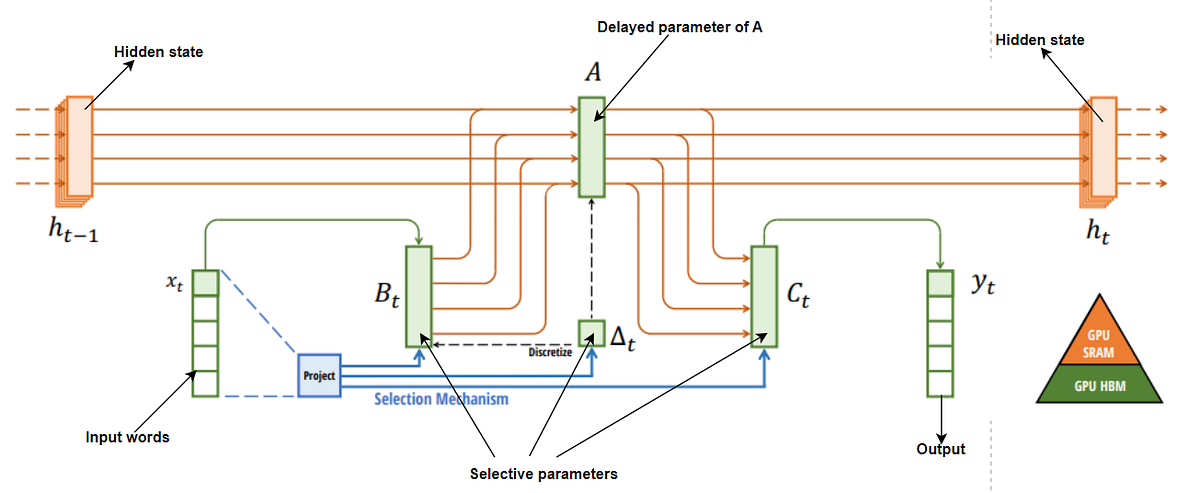
\includegraphics[width=\linewidth]{results/mamba_ssd_s6.png}
    \caption{Structured SSMs map each channel through a higher-dimensional
    latent state; the selective variant makes parts of the transition
    input-dependent. The diagram illustrates the architectural mechanism,
    not measured relay speed.}
    \label{fig:mamba_ssd_s6}
\end{figure}

\textbf{Mamba-2 (SSD)} \cite{DaoGu2024TransformersSSM} expresses the same
recurrence through structured semiseparable matrix operations, allowing
chunked batched computation with state hand-off between chunks. This supplies
algorithmic parallelism and favorable long-sequence scaling. It does not imply
lower measured end-to-end relay latency on the short-window experiment, and it
does not establish that SSMs generally outperform attention.

\subsection{State Space Models for Signal Processing}
\label{sec:state-space-models-for-signal-processing}

Classical signal processing already uses state-space descriptions in Kalman
and Wiener filtering. Neural SSMs extend that vocabulary with learned
transitions and, in selective variants, input-dependent updates. Their
relevance increases when observations are coupled across time. Architecture
comparisons in this thesis remain conditioned on parameter budget, context,
seed, and optimization; equal parameter count does not remove width, depth,
state-size, context, or training confounds.

\section{Theoretical Foundations: Channel Models}
\label{sec:theoretical-foundations-channel-models}

The canonical analytic reference is Gray-coded QPSK over coherent i.i.d.\
Rayleigh fast fading. The AWGN/BPSK expressions below are retained as
calibration and companion special cases, not as a replacement canonical model.

\subsection{AWGN Channel: Theoretical Analysis}
\label{sec:awgn-channel-theoretical-analysis}

The real AWGN companion model is
\begin{equation}\protect\phantomsection\label{eq:awgn-channel}
y=x+n,
\qquad
n\sim\mathcal N(0,\sigma^2),
\qquad
\sigma^2=\frac{P_s}{\mathrm{SNR}_{\mathrm{linear}}}.
\end{equation}

\subsubsection{Single-hop BER}\label{sec:awgn-single-hop-ber}

For unit-power BPSK under this real-noise convention,
\begin{equation}\protect\phantomsection\label{eq:awgn-ber}
P_e^{\mathrm{AWGN}}
=
Q(1/\sigma)
=
Q(\sqrt{\mathrm{SNR}})
=
\frac12\mathrm{erfc}\!\left(\sqrt{\frac{\mathrm{SNR}}2}\right).
\end{equation}
This differs in notation from the textbook \(Q(\sqrt{2E_b/N_0})\) only because
the implemented real variance is \(P_s/\mathrm{SNR}\), so
\(E_b/N_0=\mathrm{SNR}/2\). The complex fading model uses half the total noise
power per real dimension.

\subsubsection{Two-hop AF BER}\label{sec:awgn-two-hop-af-ber}

For the variable-gain background model with equal hop SNR \(\gamma\),
\begin{equation}\protect\phantomsection\label{eq:af-snr-eff}
\mathrm{SNR}_{\mathrm{eff}}^{\mathrm{AF}}
=
\frac{\gamma^2}{2\gamma+1},
\end{equation}
\begin{equation}\protect\phantomsection\label{eq:af-p-eff}
P_e^{\mathrm{AF}}
=
Q\!\left(\sqrt{\mathrm{SNR}_{\mathrm{eff}}^{\mathrm{AF}}}\right),
\end{equation}
and, at high SNR,
\begin{equation}\protect\phantomsection\label{eq:gamma-high-snr}
\mathrm{SNR}_{\mathrm{eff}}^{\mathrm{AF}}
\approx
\frac{\gamma}{2}.
\end{equation}
These expressions remain analytical background and are not the simulated
fixed-gain AF closed form.

\subsubsection{Two-hop DF BER}\label{sec:awgn-two-hop-df-ber}

For independent equal-BER hops,
\begin{equation}\protect\phantomsection\label{eq:df-ber-awgn}
P_e^{\mathrm{DF}}
=
P_{e,1}+P_{e,2}-2P_{e,1}P_{e,2},
\end{equation}
\begin{equation}\protect\phantomsection\label{eq:equal-hop-snr}
P_e^{\mathrm{DF}}=2P_e(1-P_e),
\end{equation}
and at high SNR,
\begin{equation}\protect\phantomsection
\label{eq:df-high-snr-two-hop-penalty}
P_e^{\mathrm{DF}}\approx 2P_e.
\end{equation}

\subsection{Rayleigh Fading Channel: Theoretical Analysis}
\label{sec:rayleigh-fading-channel-theoretical-analysis}

The canonical hop model is
\begin{equation}\protect\phantomsection\label{eq:rayleigh-channel}
y=hx+n,
\qquad
h\sim\mathcal{CN}(0,1),
\qquad
n\sim\mathcal{CN}(0,\sigma^2),
\end{equation}
with
\begin{equation}\protect\phantomsection\label{eq:rayleigh-pdf}
f_{|h|}(r)=2re^{-r^2},
\qquad
r\ge0,
\end{equation}
and \(\mathbb E[|h|^2]=1\). Under coherent equalization the instantaneous SNR
is proportional to \(|h|^2\).

\subsubsection{Single-hop BER}\label{sec:rayleigh-single-hop-ber}

For coherent binary detection, averaging over the exponential instantaneous
SNR gives \cite[Eq.~14-4-15]{ProakisSalehi2008DigitalComm}
\begin{equation}\protect\phantomsection\label{eq:rayleigh-ber}
P_e^{\mathrm{Rayleigh}}
=
\frac12
\left(
1-\sqrt{\frac{\bar\gamma_b}{1+\bar\gamma_b}}
\right),
\end{equation}
where \(\bar\gamma_b=E_b/N_0\). Gray-coded QPSK has the same per-bit
expression as coherent BPSK at the same \(E_b/N_0\). Because the canonical
plots use \(E_s/N_0\) and QPSK carries two bits per symbol,
\(\bar\gamma_b=(E_s/N_0)/2\). At high SNR,
\begin{equation}\protect\phantomsection\label{eq:rayleigh-ber-approx}
P_e^{\mathrm{Rayleigh}}
\approx
\frac{1}{4\bar\gamma_b}.
\end{equation}
Deep fades therefore produce the familiar first-order Rayleigh decay. This is
channel-model background, not evidence that a learned relay creates additional
diversity.

\subsubsection{Two-hop DF BER}\label{sec:rayleigh-two-hop-df-ber}

For independent hops and the symbol-wise composition used in the canonical
calibration,
\begin{equation}\protect\phantomsection\label{eq:df-ber-rayleigh}
P_e^{\mathrm{DF,Rayleigh}}
=
2P_e^{\mathrm{Rayleigh}}
\left(1-P_e^{\mathrm{Rayleigh}}\right).
\end{equation}

\section{Channel Coding: Convolutional Codes and Trellis Decoding}
\label{sec:channel-coding-background}

The supplementary coded/resource study departs from the uncoded canonical
benchmark. It should not be treated as a fifth layer of the information
ladder, and conclusions from its selected code, frame, modulation grid, and
channel are not universal coding claims.

\subsection{Convolutional Encoding: Rate and Constraint Length}
\label{sec:convolutional-encoding}

A rate-\(k/n\) convolutional encoder maps \(k\) input bits to \(n\) coded bits
per trellis step \cite{ProakisSalehi2008DigitalComm}:
\begin{equation}
R=\frac{k}{n}.
\end{equation}
For \(k=1\) and constraint length \(K\), the code trellis has
\begin{equation}
S=2^{K-1}
\end{equation}
states. Zero-tail termination appends \(K-1\) zeros to return the encoder to
the all-zero state.

\subsection{Maximum-Likelihood Sequence Decoding: The Viterbi Algorithm}
\label{sec:viterbi-decoding-background}

For a known convolutional code on a memoryless channel, Viterbi decoding finds
the minimum-metric valid codeword path by add--compare--select recursion
\cite{Forney1972MLSE,ProakisSalehi2008DigitalComm}:
\begin{equation}
\hat{\mathbf c}
=
\arg\min_{\mathbf c\in\mathcal C}
\sum_k\lVert y_k-x(c_k)\rVert^2.
\end{equation}

This \emph{code-trellis decoder} is distinct from Viterbi MLSE for channel
memory. For an \(L\)-tap channel and constellation size \(M\), channel-memory
MLSE has \(M^{L-1}\) states and evaluates \(M^L\) branches per symbol. A
model-aware MLSE remains the relevant classical detector when the channel has
memory; memory invalidates memoryless slicing, not classical processing as a
class.

\subsection{Soft-Decision Decoding: The Forward--Backward (BCJR) Algorithm}
\label{sec:bcjr-background}

BCJR \cite{BCJR1974MAP} computes symbol or bit posteriors using forward and
backward recursions:
\begin{equation}
P(s_{k-1}=s',s_k=s\mid\mathbf y)
\propto
\alpha_{k-1}(s')\,
\gamma_k(s',s)\,
\beta_k(s).
\end{equation}
Viterbi selects a most likely sequence, whereas BCJR supplies marginal APPs
and can minimize symbol or bit error for the specified trellis model.
Convolutional-code BCJR and channel-memory BCJR use the same
dynamic-programming idea on different trellises and should not be conflated. A
finite-pilot least-squares channel estimate is a point estimate, not literally
a Bayesian posterior unless a posterior model is explicitly defined.

\subsection{Puncturing, Spectral Efficiency, and Rate Adaptation}
\label{sec:puncturing-background}

With code rate \(R\) and constellation size \(M\), nominal spectral efficiency
is
\begin{equation}
\eta=R\log_2 M
\qquad [\text{bits/symbol}].
\end{equation}
Puncturing raises the effective rate by deleting a periodic subset of coded
bits and treating the missing positions as erasures at the decoder. Goodput
additionally accounts for frame failure:
\begin{equation}
G=\eta(1-\mathrm{FER})
\qquad [\text{information bits/symbol}].
\end{equation}
These quantities motivate resource-aware comparison, but they do not prescribe
a unique relay architecture for higher-order modulation. Joint
classification, regression, probabilistic soft-symbol, hierarchical, and
other formulations remain possible; this thesis does not establish a
canonical higher-order learned relay.